\lstset{breaklines=true, frame=single, language=Python, numbers=left, basicstyle=\ttfamily}
\chapter{PhononNeutron}\label{app:software}
During the thesis, a selection of Python classes were developed with the intention of generalizing some of the tasks required to get the correct neutron weights out of simulations. While software such as MDANSE \cite{Goret2017} does a good job with respect to molecular dynamics, I wanted something focussed on analyzing phonons specifically from different levels of theory (MD and `Frozen Phonons'). The code be found at \url{https://github.com/tejsner/phonon_neutron} and features two modules

\begin{enumerate}
    \item md\_tools.py
    \item phonopy\_tools.py
\end{enumerate}

\subsection{md\_tools.py}
This module is used to perform various task on molecular dynamics trajectories as obtained from VASP. VASP trajectories are saved in \texttt{XDATCAR} files, which can be analysed, for example, in the following way:

\vspace{1em}
\begin{lstlisting}
from md_tools import VaspMD
md_data = VaspMD('XDATCAR', dt=1)
md_data.compute_velocity()
md_data.compute_temperature()
md_data.compute_pdf()
md_data.compute_dos(sigma=0.5)
\end{lstlisting}
\vspace{1em}

\noindent Line 1 simply imports the module, line 2 reads the VASP trajectory and lines 3-6 computes velocity, temperature, the pair distribution function and the phonon density of states with a Gaussian smearing width of $\sigma = \SI{0.5}{\milli\eV}$. Everything is now saved in the \texttt{md\_data} object, and can be plotted, for example, using matplotlib in the following way:

\vspace{1em}
\begin{lstlisting}
import matplotlib.pytplot as plt
# temperature
plt.figure()
plt.plot(md_data.vtime, md_data.temperature)
# PDF
plt.figure()
plt.plot(md_data.pdf_x, md_data.pdf)
# DOS
plt.figure()
plt.plot(md_data.omega, md_data.dos)
\end{lstlisting}
\vspace{1em}

\noindent Many additional features are present in this module and can be found by inspecting the code. A current limitation is that it only contains neutron cross sections for the atomic species used in this thesis (La, Sr, Cu, O), but it is a fairly simple procedure to add scattering lengths at the top of \texttt{md\_tools.py}.

\subsection{phonopy\_tools.py}
This module contains a number of helper functions used to manipulate output from a Phonopy \cite{Togo2015, phonopywebsite} calculation. In particular, I wanted easy access to neutron-weighted band structure plotted in different ways as shown throughout this thesis (in particular chapter \ref{ch:lowen}). In order for the code to load Phonopy data, we require two files

\begin{enumerate}
    \item \texttt{phonopy\_disp.yaml}: Contains information about the input structure and phonon calculation.
    \item \texttt{FORCE\_SETS}: Contains the force constants obtained from DFT calculations.
\end{enumerate}

\noindent With those files, neutron weighted band structure plots can be generated in the following way

\vspace{1em}
\begin{lstlisting}
from phonopy_tools import PhonopyNeutron
import matplotlib.pyplot as plt
f, ax = plt.subplots()
ph_data = PhonopyNeutron('phonopy_disp.yaml', 'FORCE_SETS')
ph_data.set_path([[0,0,0],[0.5,0.5,0],[1,0,0],[0,0,0]])
ph_data.set_labels(['$\Gamma$', 'X', 'M', '$\Gamma$'])
ph_data.compute_bands()
ph_data.compute_neutron_bands()
ph_data.plot_neutron_bands(ax, plotype='lines', sigma=0.2)
\end{lstlisting}
\vspace{1em}

\noindent Line 1 imports the module, and line 4 imports the Phonopy data. In order to get the band structure, it is necessary to set the path in reciprocal space that you want to plot as shown in line 5. The coordinates are here with respect to the input cell, so not necessarily the primitive cell. Line 5 simply labels these paths, line 6 and 7 computes the bands and line 8 plots them. A different option is to plot in 2 dimensions of $\bm{Q}$ at a selected energy as we also saw in chapter \ref{ch:lowen}. An example of how to get this plot is:

\vspace{1em}
\begin{lstlisting}
from phonopy_tools import PhonopyNeutron, get_xy_colormap
import matplotlib.pyplot as plt
ph_data = PhonopyNeutron('phonopy_disp.yaml', 'FORCE_SETS')
cmap_data = lco.get_sqw_xy([1,5,-1,3], 100, 100)
x, y, I = get_xy_colormap(cmap_data, 9, sigma=1)
plt.pcolor(x, y, I)
\end{lstlisting}
\vspace{1em}

\noindent We load the modules in line 1, and the Phonopy data in line 3. In line 4, we generate the $S(\bm{Q},\omega)$ in a grid where $Q_x$ ranges from 1 to 5 and $Q_y$ ranges from -1 to 3 with a grid size of 100 in each direction. The evaluation of this can be quite slow, so start with a small grid size. Finally, the \texttt{get\_xy\_colormap()} function uses this data to generate a colormap at a certain energy with some fixed resolution $\sigma$ (in meV).

% \chapter{Structural Transformation Matrices}

% Conventional Cells (Bmab and P4$_2$/ncm are identical so this transformation is the identity)

% \[
% \text{I4/mmm} \quad 
% \begin{pmatrix}
% 1 & \bar{1} & 0 \\
% 1 & 1 & 0 \\
% 0 & 0 & 1
% \end{pmatrix}
% \quad \text{Bmab}
% \]

% \noindent Primitive Cells

% \[
% \text{I4/mmm} \quad 
% \begin{pmatrix}
% 1 & 1 & 0 \\
% 1 & \bar{1} & 0 \\
% 1 & 0 & \bar{1}
% \end{pmatrix}
% \quad \text{Bmab} \quad
% \begin{pmatrix}
% 1 & 0 & 1 \\
% 0 & 1 & 0 \\
% \bar{1} & 0 & 1
% \end{pmatrix} 
% \quad \text{P4}_2\text{/ncm}
% \]

% \chapter{Additional Data}
% This appendix contains plots and analysis that would be distracting in the main text, but are important to reference in any thorough investigation.

% \chapter{VASP Inputs}\label{app:vasp}

% \begin{figure}
%     \centering
%     \begin{lstlisting}[basicstyle=\footnotesize\ttfamily, frame=single]
%     ENCUT = 520 # 1.3x suggested value from O POTCAR, 800 for phonons
%     EDIFF = 1E-5 # 1E-8 for phonons
%     ALGO = NORMAL
%     PREC = Accurate
%     ADDGRID = .FALSE.
%     LREAL = Auto # Switch to .FALSE. for phonons
    
%     GGA = PS # PBESol functional, PE switches to default PBE
    
%     ISPIN = 2
%     MAGMOM = 1 -1 1 -1 24*0 # AFM structure
    
%     IBRION = -1 # Single point calculation
%     NSW = 0     # Number of ionic steps
    
%     ISMEAR = 0
%     SIGMA = 0.1
    
%     LDAU= .TRUE. # Enable LDA+U with U=8eV and J=0.8eV
%     LDAUTYPE = 4 # No exchange splitting
%     LDAUL = 2 -1 -1 # only on Cu d states
%     LDAUU = 8 0 0 
%     LDAUJ = 0.8 0 0
%     \end{lstlisting}
%     \caption[VASP: Typical INCAR]{Typical INCAR for VASP simulations.}
%     \label{fig:incar}
% \end{figure}

\chapter{Low energy phonons, additional plots}\label{app:lowen_plots}
This appendix contains the plot and fits used to compare low energy phonons with simulation data in chapter \ref{ch:lowen}. Figures \ref{fig:flatcone_phonons_400T_raw}, \ref{fig:flatcone_phonons_220T_raw}, \ref{fig:flatcone_phonons_400L_raw} and \ref{fig:flatcone_phonons_220L_raw} is data obtained from interpolation of FlatCone data in various directions. Figures \ref{fig:flatcone_phonons_dispersion_simulation_e1}, \ref{fig:flatcone_phonons_dispersion_simulation_e2}, \ref{fig:flatcone_phonons_dispersion_simulation_e3}, \ref{fig:flatcone_phonons_dispersion_simulation_e4} and \ref{fig:flatcone_phonons_dispersion_simulation_e5} show the comparison of this data with simulations in various structural and electonic phases.

\begin{figure}
    \centering
    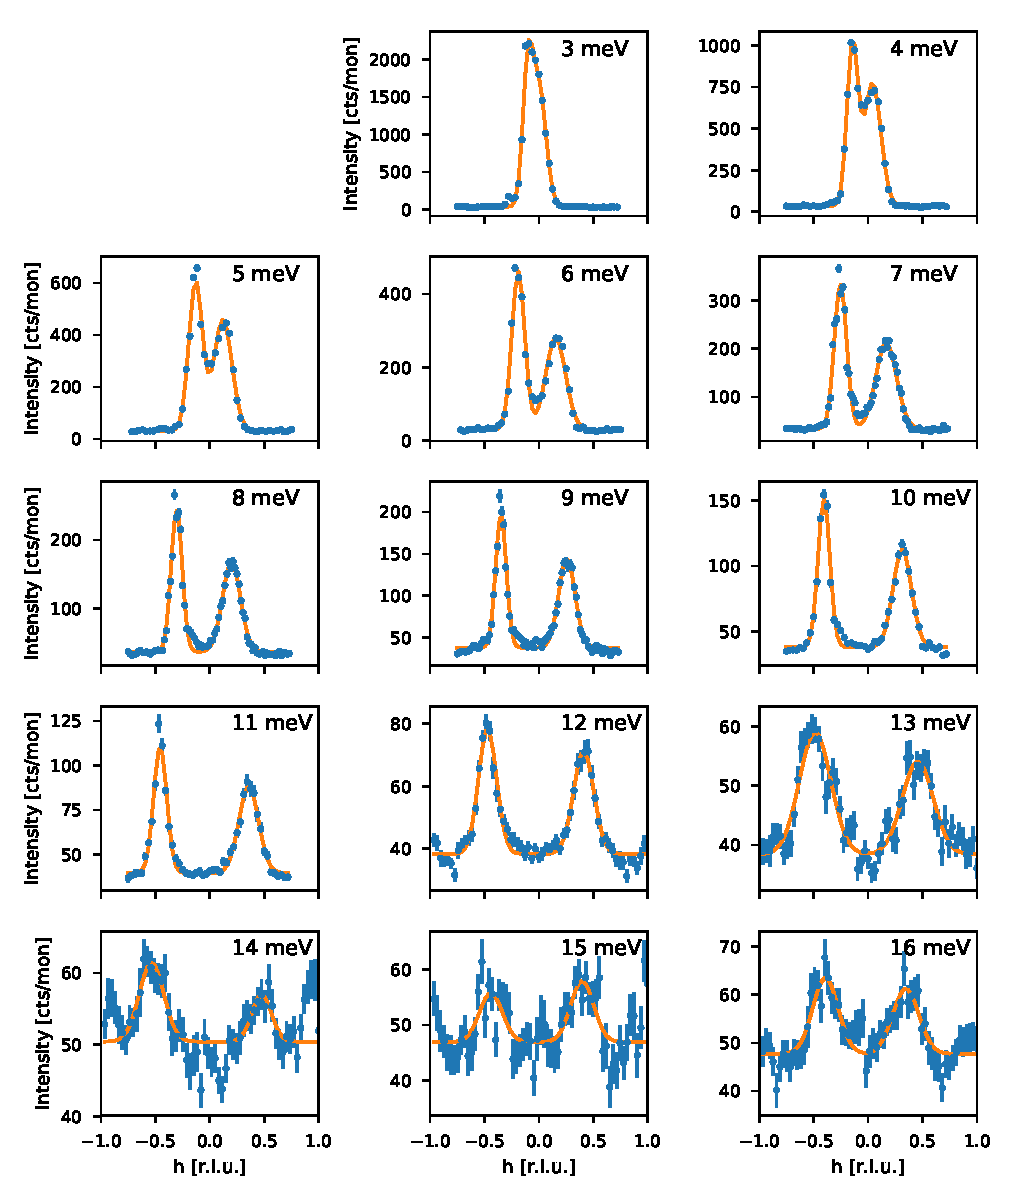
\includegraphics[width=\textwidth]{fig/lowen/fits_400T.pdf}
    \caption[400T flatcone raw data]{Interpolated data from FlatCone measurements of \LSCOOsix{} taken around the (400) peak in the transverse direction. Fits are two Gaussians.}
    \label{fig:flatcone_phonons_400T_raw}
\end{figure}

\begin{figure}
    \centering
    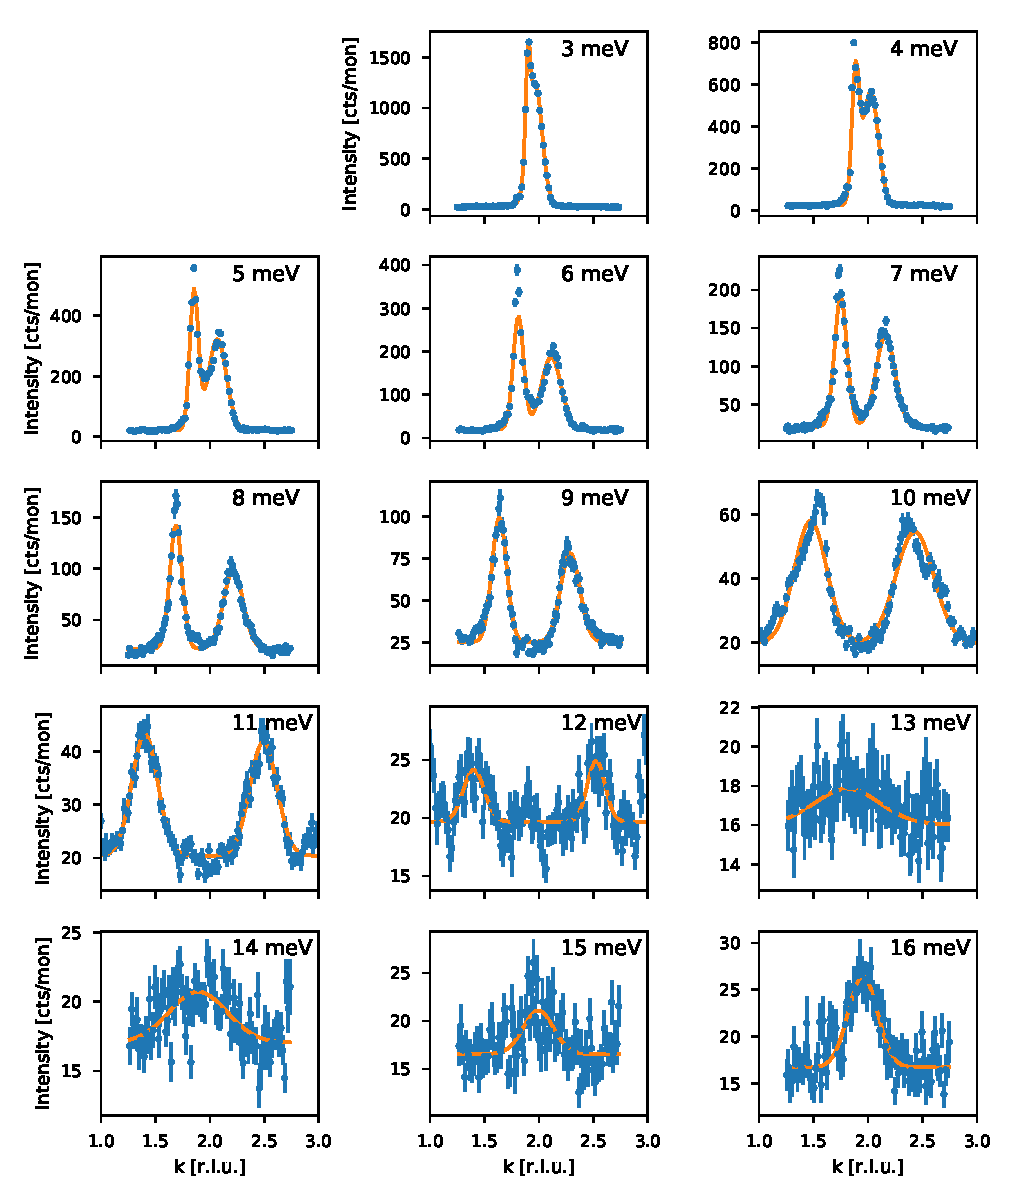
\includegraphics[width=\textwidth]{fig/lowen/fits_220T.pdf}
    \caption[220T flatcone raw data]{Interpolated data from FlatCone measurements of \LSCOOsix{} taken around the (200) peak in the transverse direction. Fits are two Gaussians.}
    \label{fig:flatcone_phonons_220T_raw}
\end{figure}

\begin{figure}
    \centering
    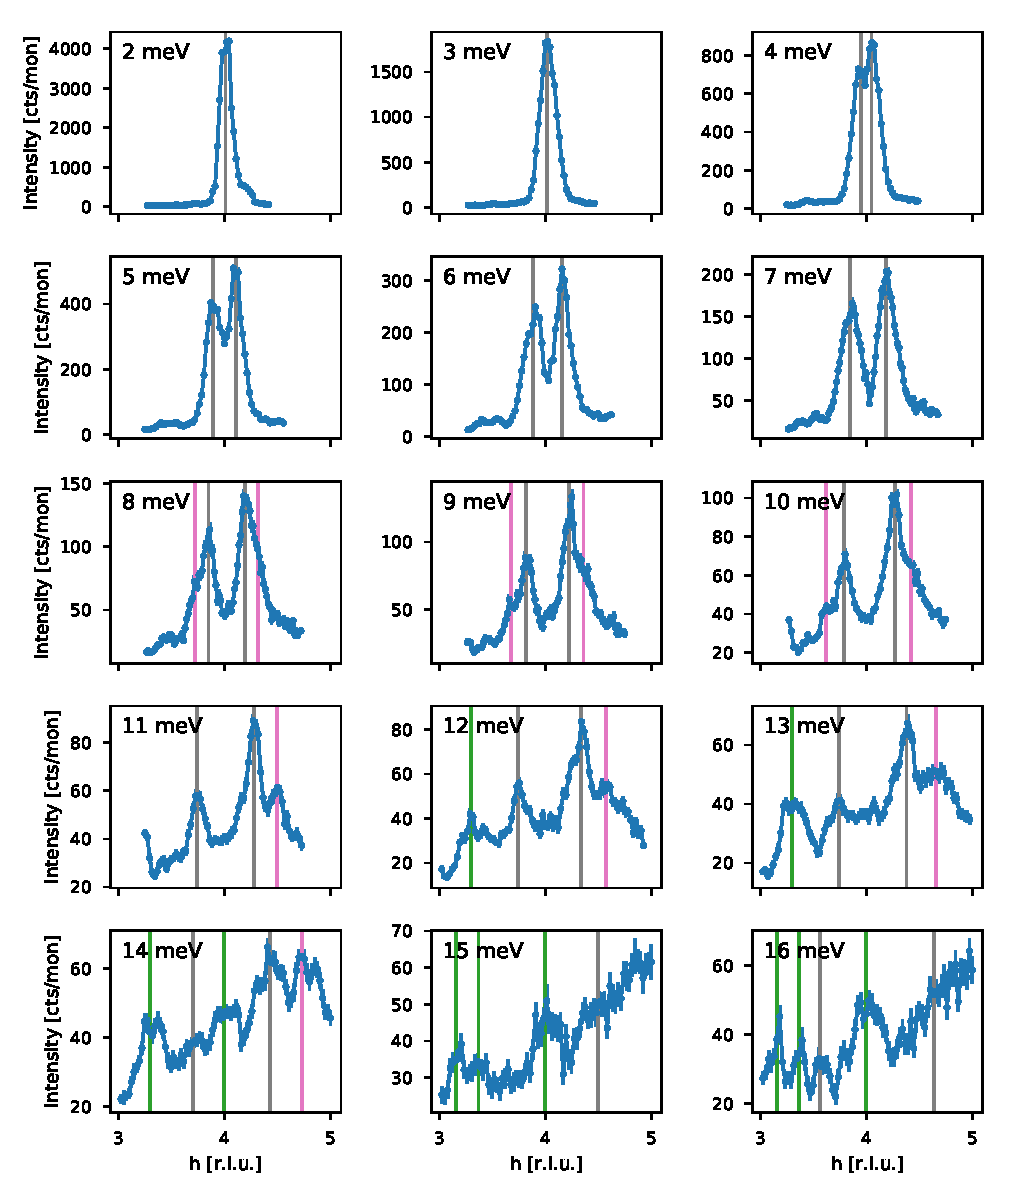
\includegraphics[width=\textwidth]{fig/lowen/fits_400L.pdf}
    \caption[400L flatcone raw data]{Interpolated data from FlatCone measurements of \LSCOOsix{} taken around the (400) peak in the longitudinal direction.}
    \label{fig:flatcone_phonons_400L_raw}    
\end{figure}

\begin{figure}
    \centering
    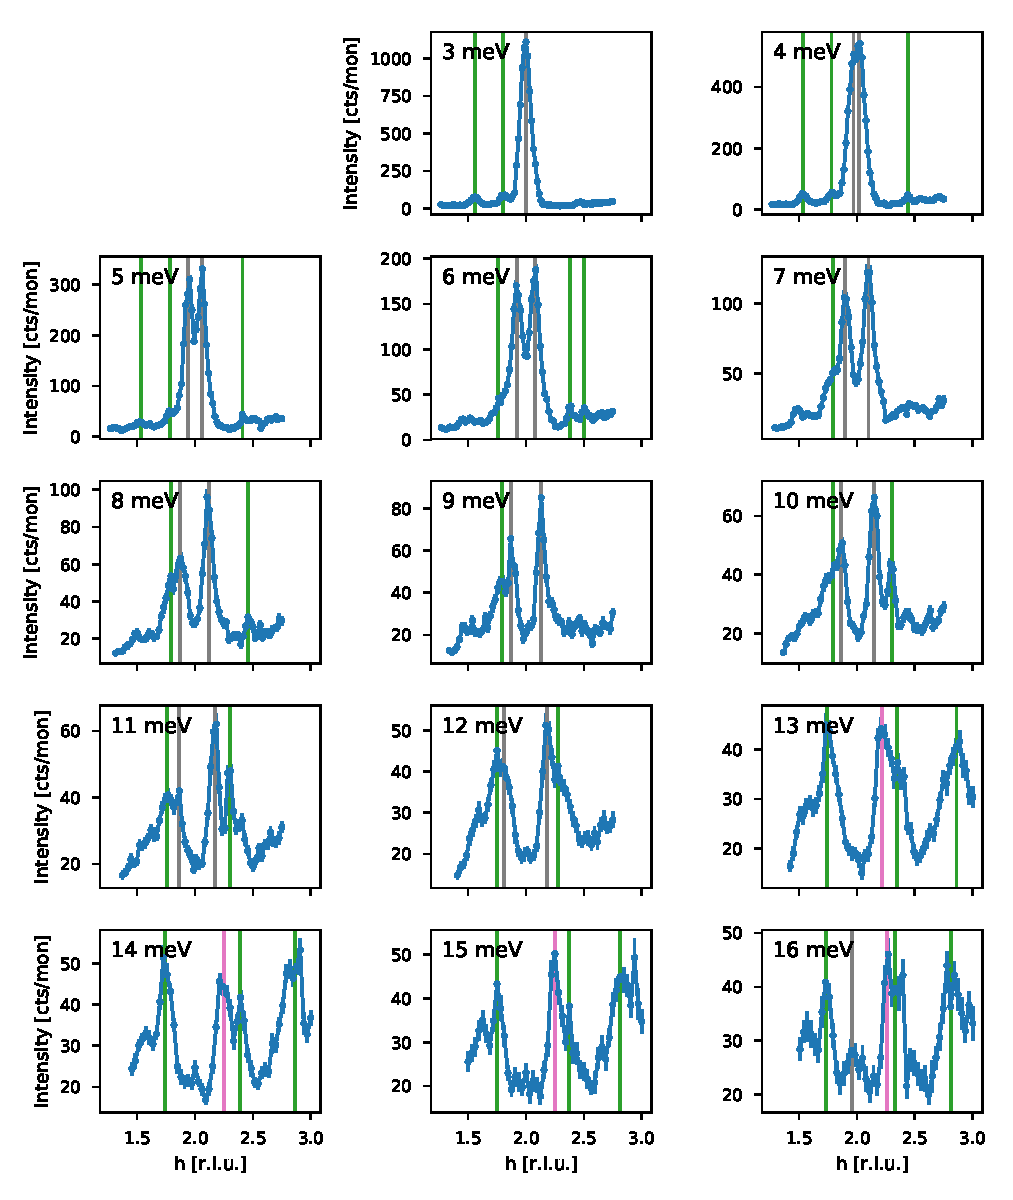
\includegraphics[width=\textwidth]{fig/lowen/fits_220L.pdf}
    \caption[220L flatcone raw data]{Interpolated data from FlatCone measurements of \LSCOOsix{} taken around the (220) peak in the longitudinal direction.}
    \label{fig:flatcone_phonons_220L_raw}    
\end{figure}

\begin{figure}[]
    \centering
    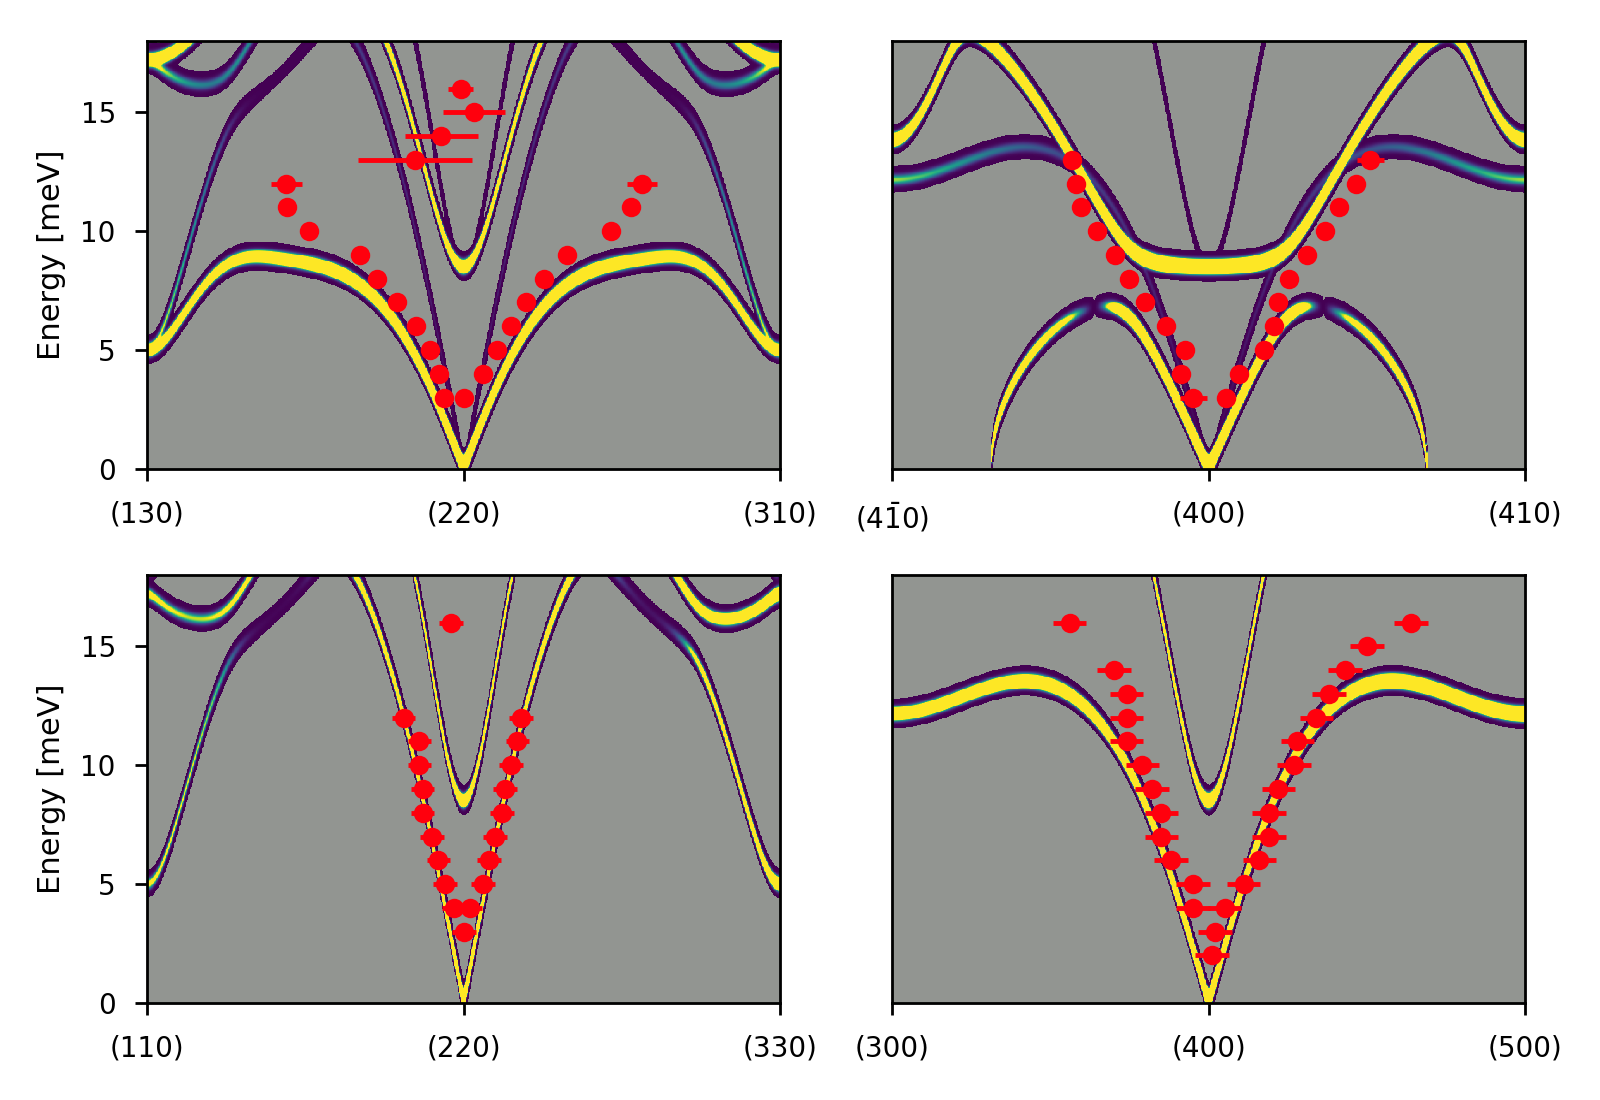
\includegraphics[width=\textwidth]{fig/lowen/flatcone_fits_simulation_htt_afm.png}
    \caption[Flatcone dispersion and neutron weighted simulation data]{Red datapoints are measured  by neutron spectroscopy using a Flatcone analyser  and lines are neutron weighted simulation data. HTT AFM simulation data.}
    \label{fig:flatcone_phonons_dispersion_simulation_e1}
\end{figure}

\begin{figure}[]
    \centering
    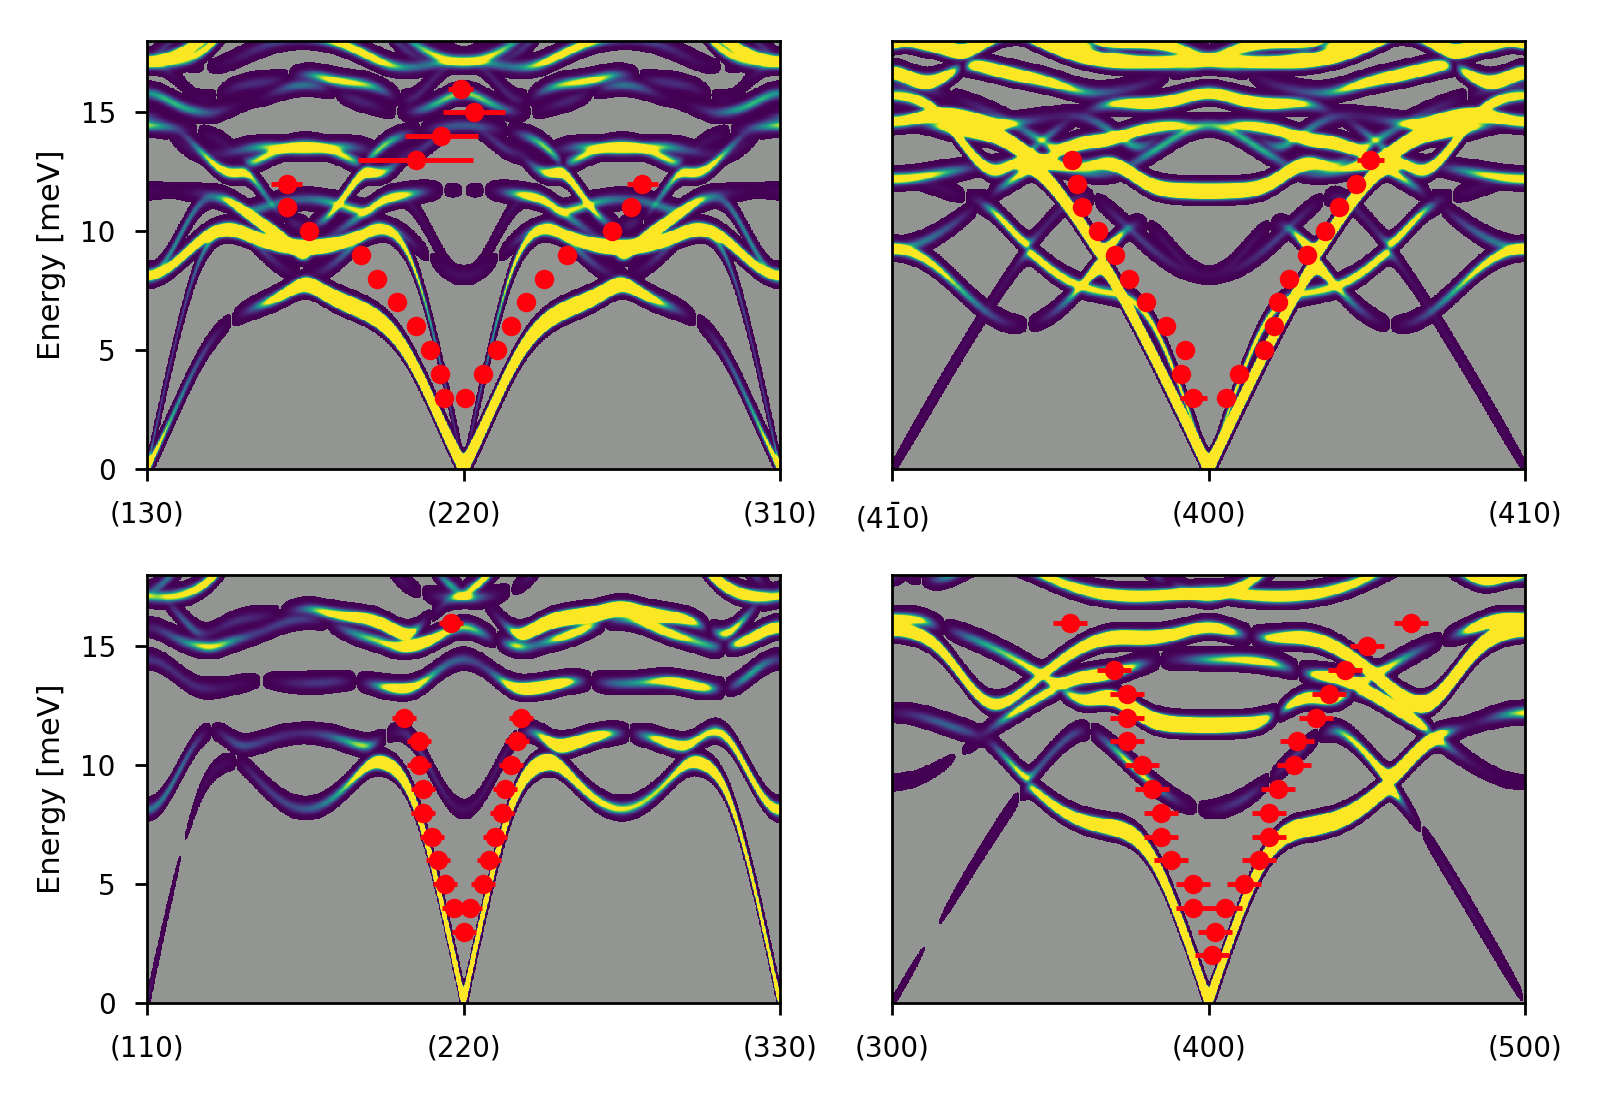
\includegraphics[width=\textwidth]{fig/lowen/flatcone_fits_simulation_ltt_afm.png}
    \caption[Flatcone dispersion and neutron weighted simulation data]{Flatcone dispersion and neutron weighted simulation data. LTT AFM simulation data.}
    \label{fig:flatcone_phonons_dispersion_simulation_e2}
\end{figure}

\begin{figure}[]
    \centering
    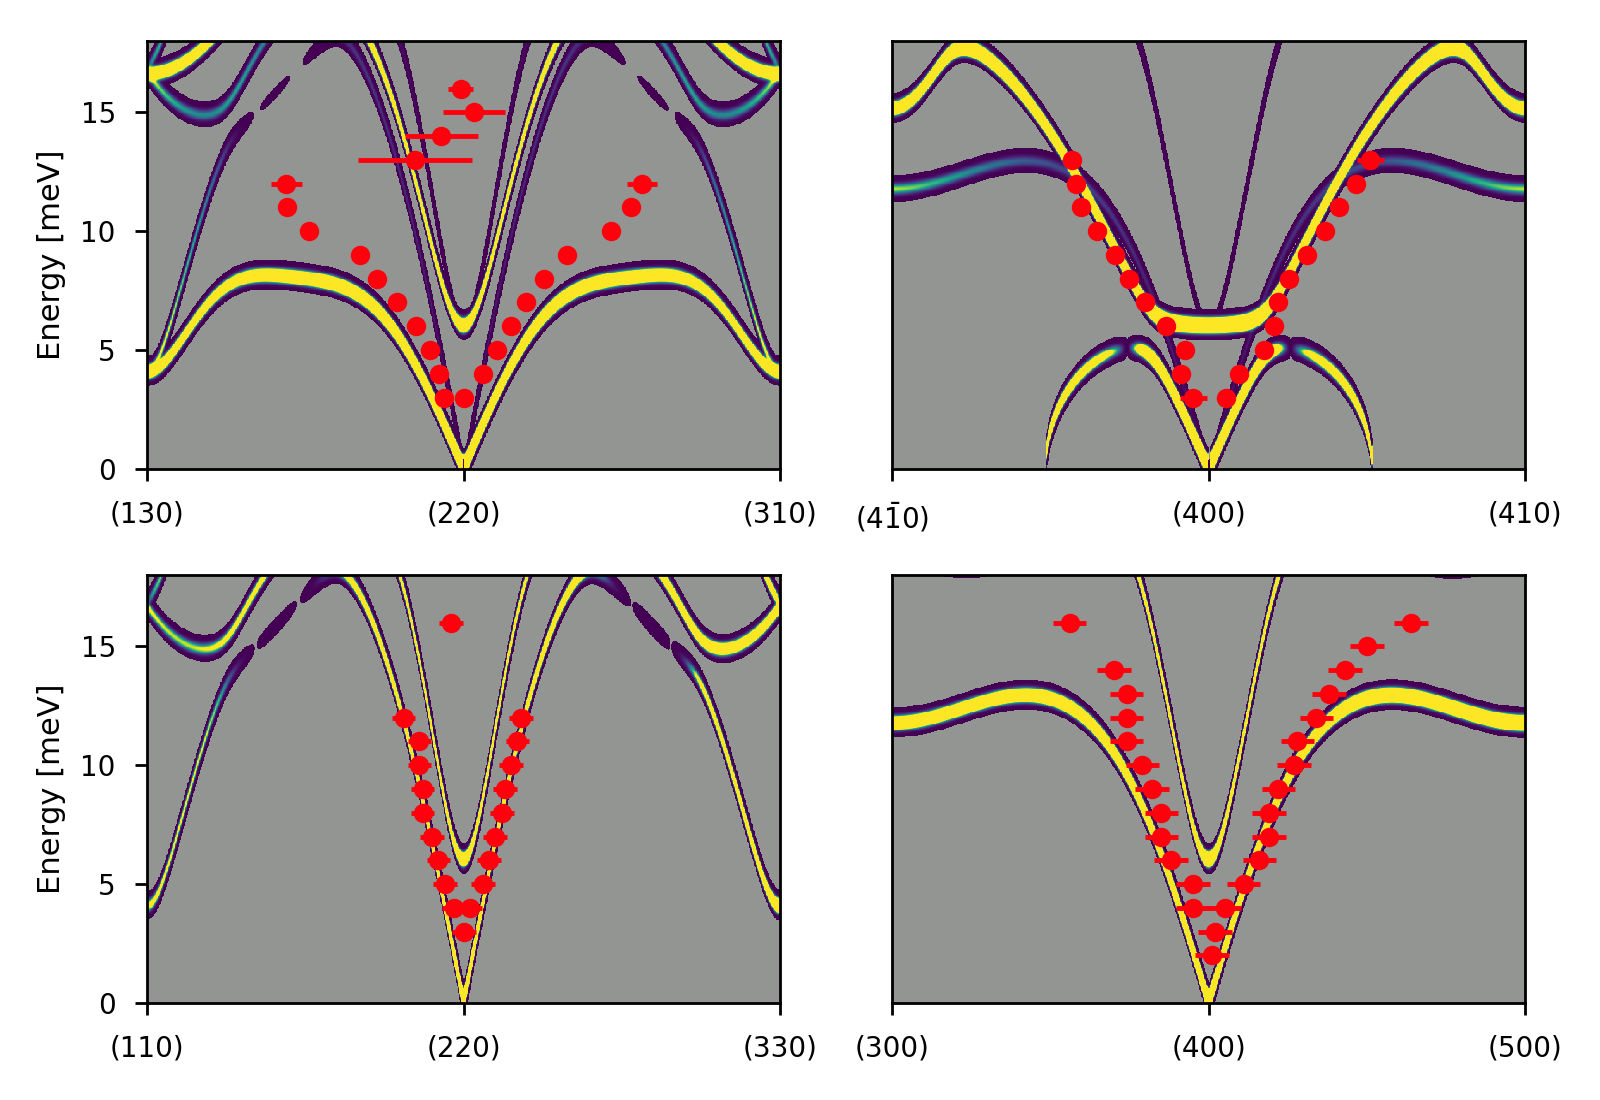
\includegraphics[width=\textwidth]{fig/lowen/flatcone_fits_simulation_htt_metal.png}
    \caption[Flatcone dispersion and neutron weighted simulation data]{Flatcone dispersion and neutron weighted simulation data. LTT AFM simulation data.}
    \label{fig:flatcone_phonons_dispersion_simulation_e3}
\end{figure}

\begin{figure}[]
    \centering
    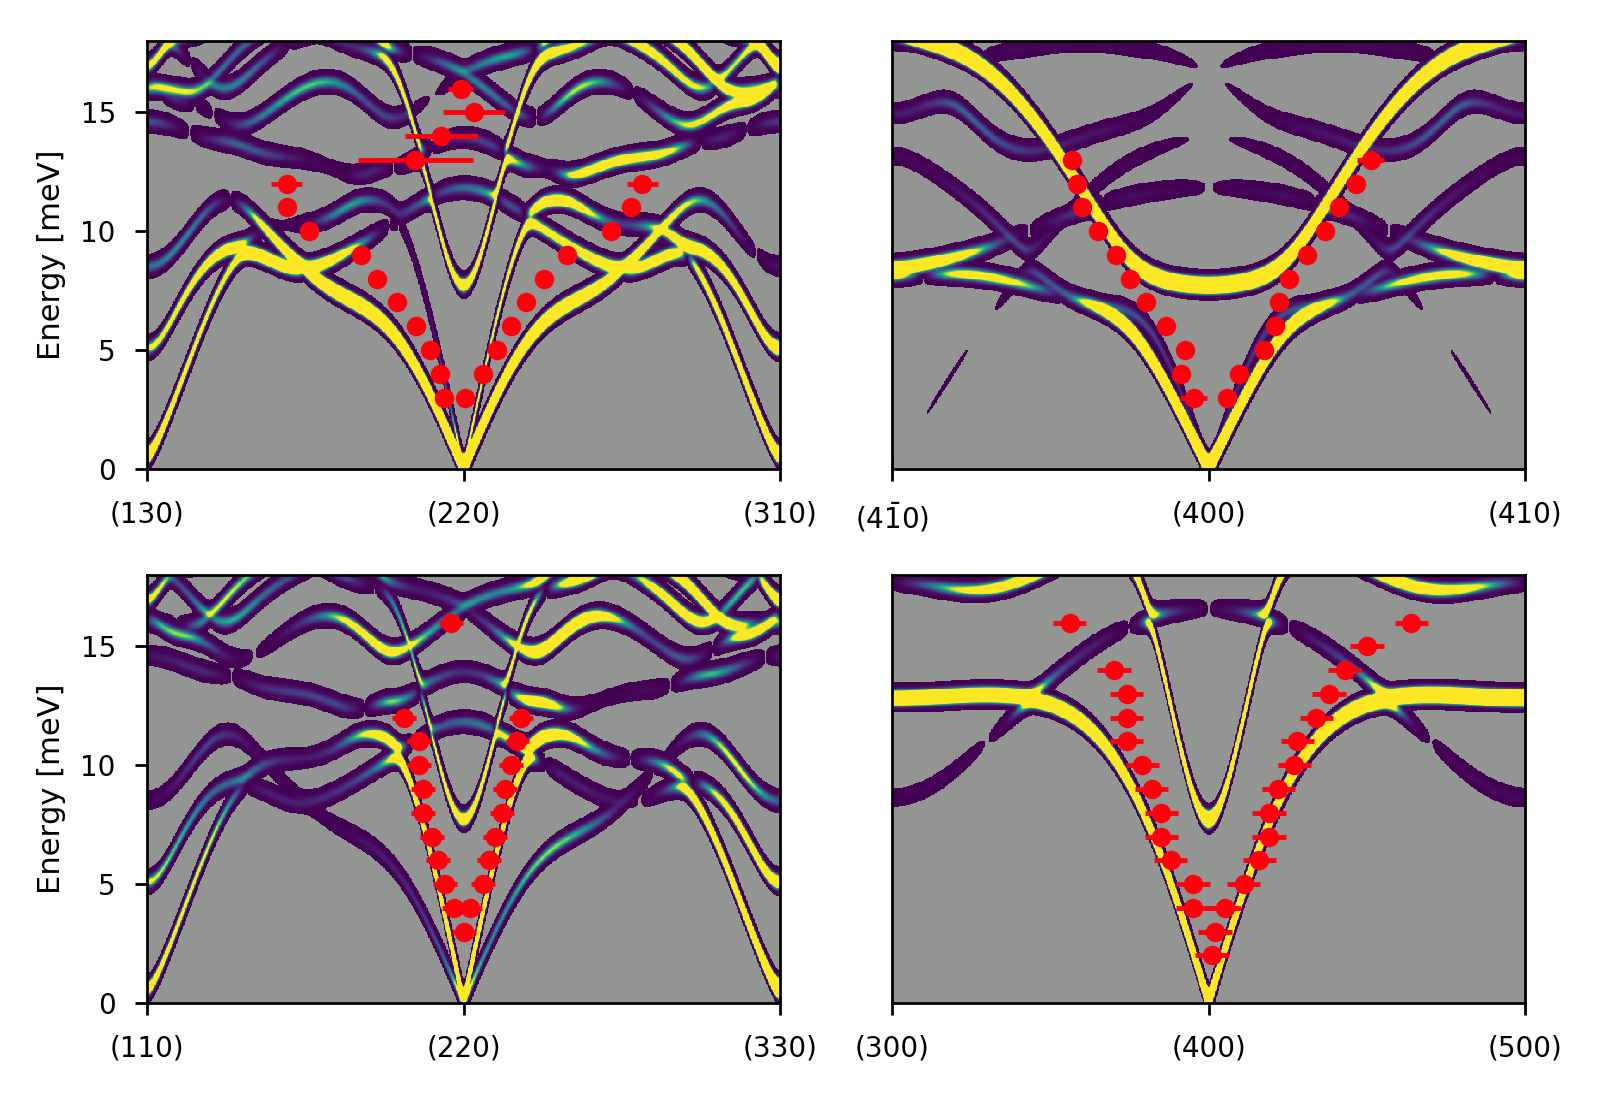
\includegraphics[width=\textwidth]{fig/lowen/flatcone_fits_simulation_lto_metal.png}
    \caption[Flatcone dispersion and neutron weighted simulation data]{Flatcone dispersion and neutron weighted simulation data. LTO metal simulation data.}
    \label{fig:flatcone_phonons_dispersion_simulation_e4}
\end{figure}

\begin{figure}[]
    \centering
    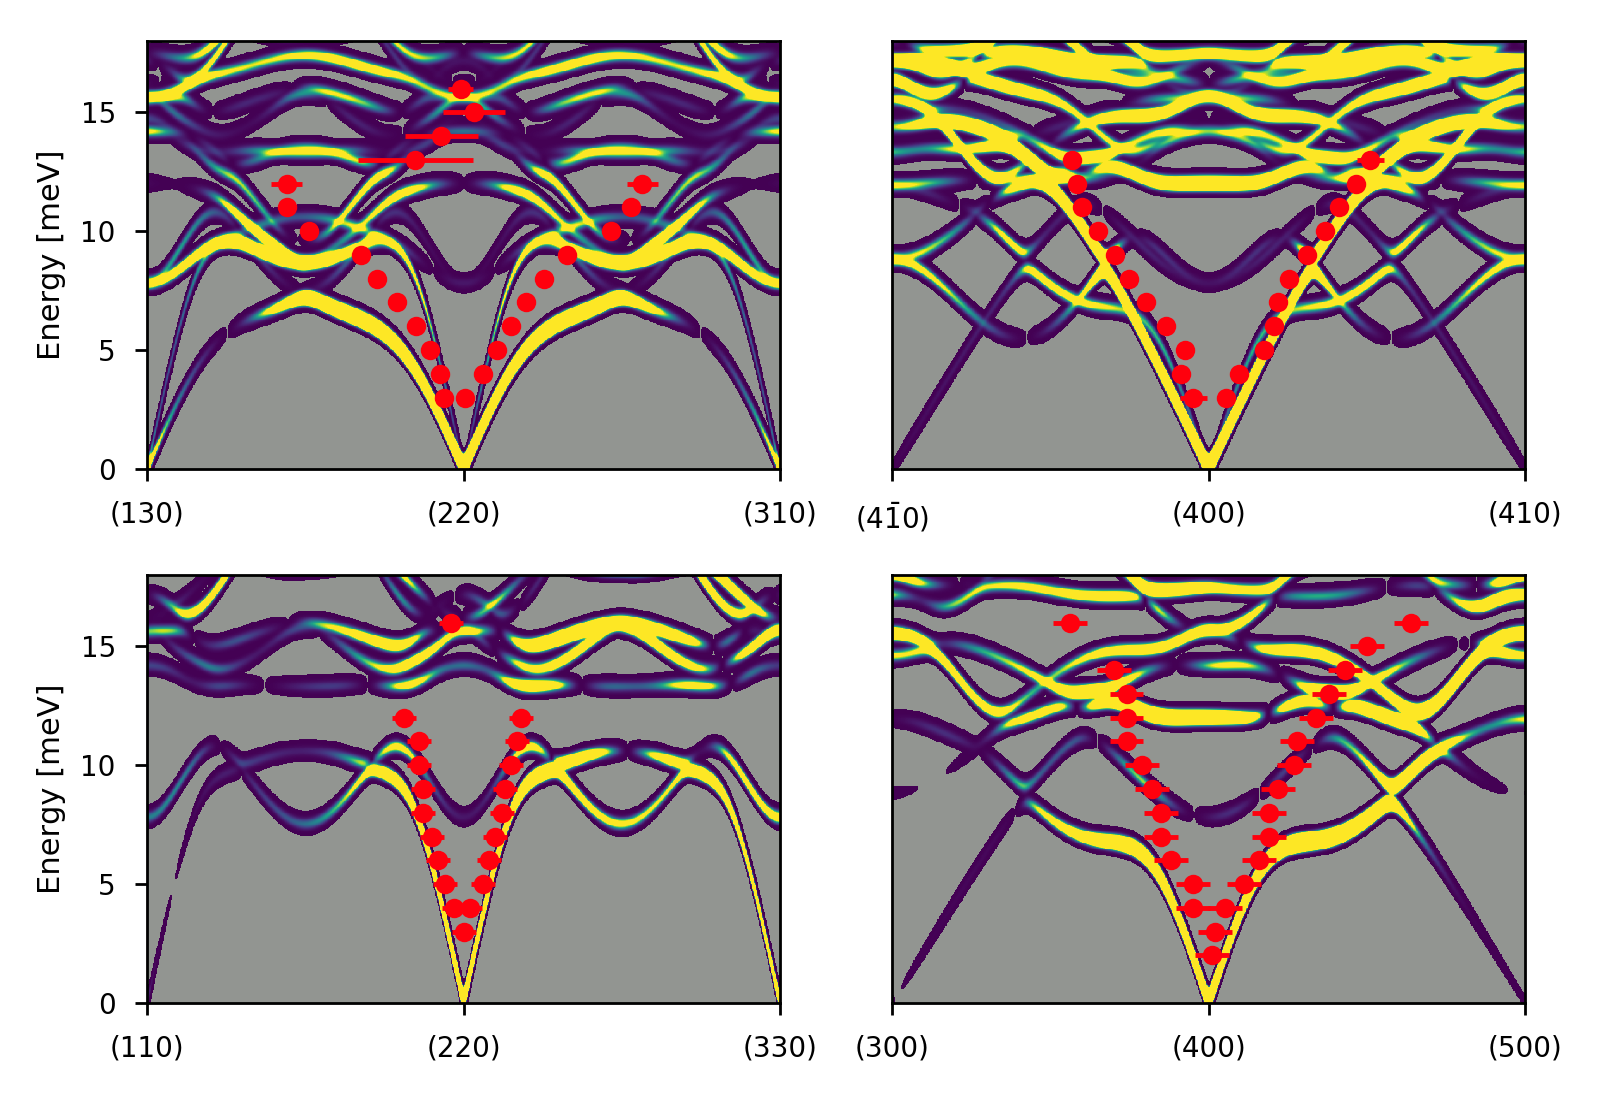
\includegraphics[width=\textwidth]{fig/lowen/flatcone_fits_simulation_ltt_metal.png}
    \caption[Flatcone dispersion and neutron weighted simulation data]{Flatcone dispersion and neutron weighted simulation data. LTT Metal simulation data.}
    \label{fig:flatcone_phonons_dispersion_simulation_e5}
\end{figure}

\chapter{Phonon DOS, additional plots}\label{app:pdos_plots}
This appendix contains additional temperatures of the density of states measurements performed in chapter \ref{ch:in4}. Figure \ref{fig:gdos_60k} contains data for \SI{60}{\kelvin} and \ref{fig:gdos_300k} contains data for \SI{300}{\kelvin}

\begin{figure}
    \centering
    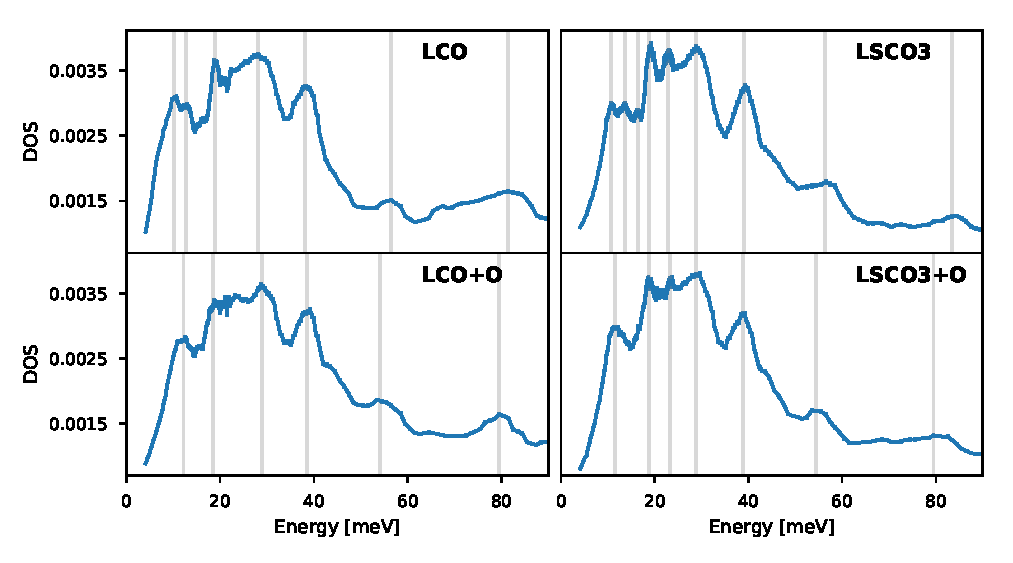
\includegraphics[width=\textwidth]{fig/gdos/in4_60K.pdf}
    \caption[gDOS at \SI{60}{\kelvin}]{Phonon density of states of all four samples at at \SI{60}{\kelvin}}
    \label{fig:gdos_60k}
\end{figure}

\begin{figure}
    \centering
    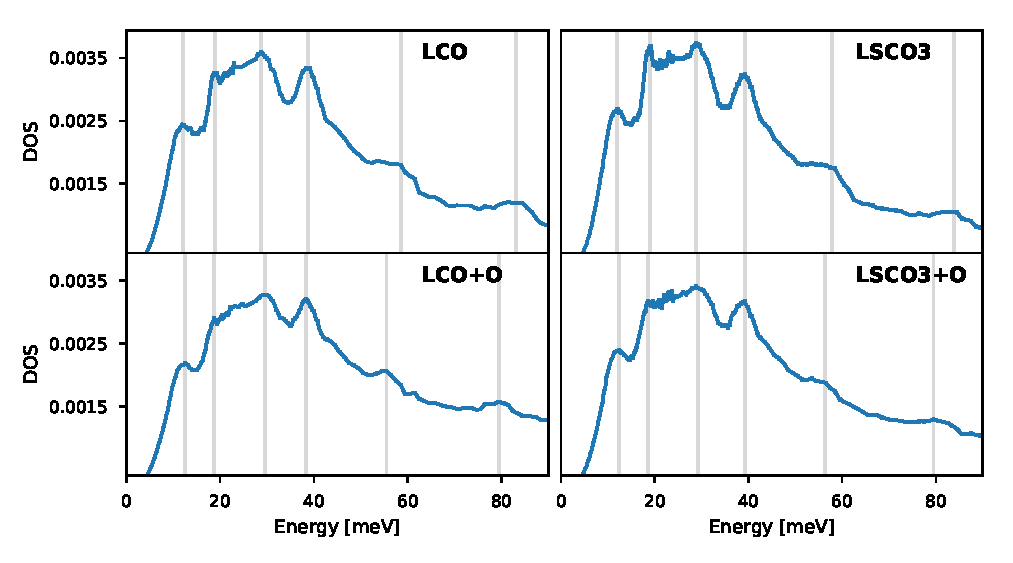
\includegraphics[width=\textwidth]{fig/gdos/in4_300K.pdf}
    \caption[gDOS at \SI{300}{\kelvin}]{Phonon density of states of all four samples at at \SI{300}{\kelvin}}
    \label{fig:gdos_300k}
\end{figure}